\documentclass{sig-alternate}
%%\documentclass[english]{hacked-sig-alternate}

\usepackage[usenames, dvipsnames]{color}
%\usepackage{times}
\usepackage{xspace}
\usepackage{textcomp}
\usepackage{wrapfig}
\usepackage{url}
\usepackage{amsmath, amssymb}
\usepackage[protrusion=true,expansion=true]{microtype}
%\usepackage{float}
\usepackage{alltt}
\usepackage{appendix}
%\usepackage{algorithm}
%\usepackage{algorithmicx}
%\usepackage{algpseudocode}
%\usepackage{texlive-science}
\usepackage{comment}
\usepackage{array,tabularx}

%\usepackage{txfonts}
\newcommand{\eat}[1]{}

\newtheorem{theorem}{Theorem}
\newtheorem{lemma}{Lemma}
\newtheorem{corollary}{Corollary}
%\theoremstyle{definition}
\newdef{example}{Example}
\newdef{definition}{Definition}

\newcommand{\naive}      {na\"{\i}ve\xspace}
\newcommand{\Naive}      {Na\"{\i}ve\xspace}

\newcommand{\jmh}[1]{{\textcolor{red}{#1 -- jmh}}}
\newcommand{\paa}[1]{{\textcolor{blue}{#1 -- paa}}}
\newcommand{\rcs}[1]{{\textcolor{green}{#1 -- rcs}}}
\newcommand{\nrc}[1]{{\textcolor{magenta}{#1 -- nrc}}}
\newcommand{\wrm}[1]{{\color{BurntOrange}{#1 -- wrm}}}

\begin{document}

%\conferenceinfo{ACM PODS}{'10 Indianapolis, IN, USA}
\title{Deterministic Concurrent Programming with Algebra}

\pdfinfo{/Title (Algebraic Programming for Parallel Asynchronous Systems)}

%%Format\titlenote{(Produces the permission block, copyright information and page numbering). For use with ACM\_PROC\_ARTICLE-SP.CLS V2.6SP. Supported by ACM.}}
%
% You need the command \numberofauthors to handle the "boxing"
% and alignment of the authors under the title, and to add
% a section for authors number 4 through n.

\numberofauthors{1}

\author{
\alignauthor William R.\ Marczak\\
\affaddr{UC Berkeley}\\
\email{wrm@cs.berkeley.edu}
}

\toappear{}

\maketitle

\begin{abstract}
Codd's idea of order-independence underlies much of the fields of query
optimization and parallel databases.  In this paper, we apply
order-independence as a programming pattern for writing correct deterministic algorithms that admit order non-determinism for increased performance by way of randomness or parallelism.
We propose a programming language for decomposing algorithms
into ``algebra'' and ``ordering,'' in the vein of Kowalski's famous ``Algorithm
= Logic + Control'' formulation.  In our language, a programmer writes a
specification in ``algebra;'' the program's performance characteristics can
then be tuned without affecting its meaning by changing only the ``ordering.''
Our
"algebra" is similar to the Bloom language for distributed systems.  In
Bloom, programmers react to an adversarial network that may reorder
messages by removing order from their code.  In contrast, our ``algebra''
forces programmers to proactively write order-independent code so that the
order may later be customized.  We present the notion of ``timelines'' as an
interface between ``algebra'' and ``ordering:'' the ``ordering'' can be any
arbitrary code that produces a ``timeline,'' whereas the ``algebra'' is
restricted to ensure that program outcomes are independent of the
``ordering.''  We formally prove this property of our language, and
demonstrate its applicability by considering a variety of case studies.
\end{abstract}

\section{Introduction}
%Our research is motivated by two hard problems in distributed systems.  First,
\wrm{show examples of the problems (not necessarily code) -- evolving state and unreliable communication}

%Distributing any system introduces nondeterminism.  For example, one may
%distribute a computation over many inexpensive, but unreliable, commodity
%machines (e.g. RAID).  The status of internet links and widely distributed
%nodes is inherently more unreliable than multiple cores on a single die, or
%multiple CPUs in a single computer.  

%We present {\bf \lang}, a foundation language for programming and
%reasoning about distributed systems.  

%We correct deficiencies in earlier attempts, and introduce a compelling notion
%of non-determinism in the language.  We specifically use non-determinism to
%reason about {\em when} a deduction becomes visible, including the possibility
%that the deduction will never be visible.  Programmers can constrain this
%non-determinism by using well-studied techniques in distributed systems, such as
%Lamport Clocks 


Traditional database systems are based on declarative query languages that
specify transformations as dataflows over an updatable store.  Such query
languages are either not expressive enough to capture common programming
constructs \wrm{like what?}, or are at best awkward to use in this fashion.
\wrm{todo: transition that explains Datalog's birth from these languages... I
don't know enough to write it} The family of logic-based database languages, of
which Datalog is the progenitor, represent expressive programming languages
that produce similar dataflow representations.  Datalog is purely deductive: a
program specifies the rules by which the derived relations are populated based
on a static database, which is never updated.  Recent programming language
research has explored the use of Datalog-based languages for expressing
distributed systems.  Because the state of any complex system evolves with its
execution, these efforts were forced to extend the Datalog model by admitting
updates, additions and deletions of the EDB.  Unfortunately, these previous
attempts were plagued with ambiguities about how and when state changes occur
and become visible, putting a heavy burden on the programmer to ensure even
simple properties, such as atomicity of updates over time.

In contrast to reasoning about state change procdurally, \lang observes
that this concept is intuitively expressed as invariants over {\em time}.  In
this work, we present a formal model of Datalog augmented with time extensions.
By reifying time as data an introducing it into the logic, \lang eliminates
previous ambiguities, ensures atomicity of updates and makes it possible to
express system invariants that can guarantee liveness properties, a key
challenge in building distributed systems.

\section{Background}
\label{sec:background}
\begin{table}
\begin{tabular}{|c|l|p{1.85in}|}
\hline
\textbf{Op} & \textbf{Name} & \textbf{Meaning} \\
\hline
\verb|<=| & \emph{merge} & lhs includes the content of rhs in the
current timestep \\
\hline
\verb|<+| & \emph{deferred merge} & lhs will include the content of rhs in the
next timestep \\
\hline
\verb|<-| & \emph{deferred delete} & lhs will not include the content of the rhs
in the next timestep \\
\hline
\verb|<|$\sim$ & \emph{async merge} & (remote) lhs will include the content of the
rhs at some non-deterministic future timestep\\
\hline
\end{tabular}
\caption{Bloom operators.}
\label{tbl:bloom-ops}
\end{table}

\begin{figure}[t]
\begin{scriptsize}
\begin{lstlisting}
class AllPaths
  include Bud

  state do
    table :link, [:from, :to, :cost]
    table :path, [:from, :to, :next_hop, :cost]
  end

  bloom :make_paths do
    path <= link {|l| [l.from, l.to, l.to, l.cost]}
    path <= (link*path).pairs(:to => :from) do |l,p|
      [l.from, p.to, l.to, l.cost + p.cost]
    end
  end
end
\end{lstlisting}
\end{scriptsize}
\caption{A Bloom program to compute the transitive closure of the
  \emph{link} relation.}
\label{fig:bloom-spaths}
\end{figure}

In this section, we briefly review the Bloom programming language and the CALM
program analysis technique.  We highlight a simple distributed protocol for
which the CALM analysis produces unsatisfactory results.

\subsection{Bloom}
\label{sec:bg-bloom}

\subsection{CALM Analysis}
\label{sec:bg-calm}

\section{Case Study}
\label{sec:case}

\wrm{Re-do case studies in Bud} \wrm{Break cart development down into
iterations} \wrm{How does the language naturally lead us to an order
independent style?  Talk about inserting all sorts of exotic stuff like queues
if we want a highly order-dependent imperative style.}


\bibliographystyle{abbrv}
\bibliography{pods}

%\appendix
%\section{Proof of Lemma 1}
\begin{proof}
%First, we prove an isomorphism between stable models, and finite prefixes of stable models.  Scan a stable model of a program timestamp by timestamp.  
We first present an algorithm for computing ultimate models, and argue that the algorithm computes exactly the stable models of the \lang program.  We then argue this algorithm can be run on our operational formalism, show how operational traces correspond with prefixes of stable models.

Any \lang program without asynchronous rules is a $\text{Datalog}_1S$ program, and the algorithm given in~\cite{tdd} computes an ultimate model in polynomial space\footnote{The class of {\em multi-seperable}~\cite{tdd-poly} \lang rules, which comprises all \lang programs $P$ with guarded asynchrony and persisted EDB, and their coordinations $\textsc{Coord}(P)$, can be executed in polynomial time.} in the size of the input.  The algorithm evalutes the program for $2^G + e$ consecutive timesteps, where $G$ is the number of instantiations of the non-temporal attributes of the program rules, using all combinations of constants in the Herbrand Universe, and $e$ is the maximum timestamp of any EDB fact.  At each step, the algorithm updates information on observed periodicities of facts.  When the algorithm terminates, any fact with a periodicity of 1 is regarded as part of the ultimate model.

For asynchronous rules, the natural distributed analog of the algorithm above simultaneously executes one instance for each node \dedalus{n}, using values of $G$ and $e$ computed from $E_{\text{\dedalus{{\scriptsize n}}}}$.  Each instance has its own local clock, which intuitively corresponds to the timestamp attribute in the model-theoretic semantics.  Nodes communicates over channels with arbitrary delay and message re-ordering.  When another node \dedalus{m} derives a fact at \dedalus{n}, it encloses its local clock value, \dedalus{t}; \dedalus{n} must consider this fact until time \dedalus{t}, in the style of Lamport Clocks.  Note that this behavior is implied by the model-theoretic semantics---remote asynchronous rules state that their deductions are visible at the destination at a time later than the body temporal attribute at the source.  Further, note that Lamport Clocks only introduce the constraint that if message $a$ ``happens before'' $b$, in other words $a$ directly or transitively causes $b$ to be sent, then $T(a) < T(b)$.  If $a$ and $b$ are concurrent, there is some execution where $T(a) \geq T(b)$.

When \dedalus{n} processes a received message, the number of constants available to \dedalus{n} may increase, and thus a node's $G$ may increase to $G'$.  Furthermore, the node may need to execute over this new fact for $2^{G'}$ additional timesteps.  If only finitely many messages are sent, this algorithm requires polynomial space.  In the case that infinitely many messages are sent, we only need to process each message $2^{G'}$ times: the maximum period of any fact is $2^{G'}$, as every incoming fact needs to have a chance (in some execution) to join with any deduction, at any time during its period, with which it is ``concurrent''.  Keeping track of the number of times we have seen each fact also requires polynomial space.  When the algorithm is done running for $2^{G'}$ steps, it pauses, waiting for new network input that it has not seen enough times.  If all nodes are paused and no outstanding messages exist, then the collection of all period 1 facts at all instances of the algorithm comprises an ultimate model.

We claim that the algorithm can generate every ultimate model---every message has the opportunity to join with another concurrent message or its transitive consequents at any point during their period, and has the opportunity to join with a causally related message during the range of times allowed by the model-theoretic asynchronous constraint (identical to the Lamport Clock condition used in the algorithm).

Note that we can execute this algorithm on our operational formalism.  Evaluating a single timestamp of a \lang program corresponds to the evaluation of a Datalog program, which is a polynomial time computation, and the Turing Machines can also maintain the necessary state about periods and message counts.
%2) Intuitively, the operational model is based on n Turing Machines, one per value of node(), which independently step sequentially through time and communicate via channels with
%non-deterministic delay.  At each timestep t they run a datalog fixpoint computation that evaluates P on ``projection(E_n, t)'' (notation needed); this takes polynomial
%time~\cite{immerman}.  At the end of this fixpoint there are three sets of relevant facts: local, synchronous facts that have timestep t+1 and become part of ``projection(E_n,
%t)'', local asynchronous facts whose timestep is chosen non-deterministically to be greater than t and become part of later timesteps, and remote asynchronous facts.  The
%timestamps in this third class of facts are chosen non-deterministically ``at the receiver'' to model delay, in a way that observes traditional causality
%restrictions~\cite{lamportclocks}.
%3) Any \lang program without  async rules is a Datalog_{1S} program, and the above intuition is captured by the algorithm given in~\cite{}, computing an ultimate model in
%polynomial space in the size of the input.  In the presence of asynchronous rules, this formalize needs to be expanded to account for the asynchronous advancement of time through
%\dedalus{successor} at each node.  The PSPACE guarantees of~\cite{} are not shown to hold for such programs, but in Appendix Foo we show that the following Lemma holds for all
%\lang programs under this model
\end{proof}

\section{Proof of Lemma 2}
\begin{proof}
We begin by assuming that \dedalus{node} contains the identifiers of each of the $n$ nodes.  Since the atemporal fragment of \lang is FO[LFP], we can represent a polynomial-time bounded Turing Machine using only atemporal rules in \lang~\cite{immerman-ptime}.  In addition to normal operations, the Turing Machine can place items into a queue---\cite{dedalus} shows how to model queues in \lang---or send messages to other nodes---modeled by an asynchronous communication rule with \dedalus{queue} in the head.  A node persists the contents of the tape across time if the queue is empty, using a rule like \dedalus{tape(\dbar{X})@next <- tape(\dbar{X}), !queue(\dbar{\_});}.  If the queue is non-empty, the computation skips a timestamp (leaving \dedalus{tape} empty), and then atomically copies the contents of \dedalus{queue} to \dedalus{tape}.  The ultimate model of this program is exactly the final contents of the tape on every node if the computation halts.  Otherwise, the program's ultimate model is empty: \dedalus{tape} facts only exist every other timestamp, and for any Turing Machine predicate \dedalus{r} we can create \dedalus{r'}, and create a mutual recursive cycle to ensure neither \dedalus{r} nor \dedalus{r'} contains facts at every timestamp:

\begin{Dedalus}
r(\dbar{X})@next <- r'(\dbar{X});
r'(\dbar{X})@next <- r(\dbar{X});
\end{Dedalus}

We can play a somewhat similar trick for \dedalus{queue} by having local messages alternate between going into \dedalus{queue} and \dedalus{queue'}.  Thus, no local queue message will be part of the ultimate model.  Remote messages will still go into \dedalus{queue}: this still leaves the case that the exact same message repeatedly arrives at a node at every timestamp forever, by chance.  We can dispense of this case by assuming the channels interconnecting the Turing Machines forbid it.
\end{proof}

\section{Proof of Lemma 3}
\begin{proof}
Our proof proceeds via construction of a two counter machine in \lang, inspired by the construction in~\cite{undecidable-datalog}. We briefly review two counter machines.  A two counter machine's state is captured in the state of its two counters (natural numbers), and in its control state.  A two counter machine has a transition function: $\delta: \Sigma \times \{=, >\} \times \{=, >\} \rightarrow \Sigma \times \{inc, dec\} \times \{inc, dec\}$

$\Sigma$ is a finite set of states (for simplicity we assume a finite subset of the natural numbers), $=$ indicates a counter is equal to zero, and $>$ indicates a counter is greater than zero.  $inc$ and $dec$ indicate that a counter should be incremented, or decremented respectively.

We represent the state of a two counter machine using the \linebreak \dedalus{cnfg(T,S,C1,C2)} relation, where \dedalus{T} represents ``time'' (note this is not the same as the timestamp attribute), \dedalus{S} is the state (in $\Sigma$), and \dedalus{C1} and \dedalus{C2} are the values of the two counters.  In order to support $inc$ and $dec$, we would like to make use of the \dedalus{succ} relation.  However, \lang conventions forbid the use of this infinite relation outside of the timestamp attribute.  Thus, we posit the \dedalus{fin\_succ(X,Y)} EDB relation, which represents a finite prefix of the successor relation.  Since it is EDB, its contents may be arbitrary.  If \dedalus{fin\_succ} is malformed, then the machine's execution may be incorrect.  In particular, our model of the machine may accept an input, whereas the actual machine would not have accepted that input.  We illustrate how to constrain the contents of \dedalus{fin\_succ} below:

\begin{Dedalus}
malformed() <- fin_succ(_,0);
malformed() <- fin_succ(X,Y), fin_succ(X,Z), Y != Z;
malformed() <- fin_succ(Y,X), fin_succ(Z,X), Y != Z;
malformed() <- fin_succ(X,Y), X >= Y;
\end{Dedalus}

For a given EDB, the two counter machine either halts in the accepting state or halts in a non-accepting state.  It cannot run forever since the EDB (in particular, the \dedalus{fin\_succ} relation) is finite.

We construct a \lang program that nondeterministically decides to either run the machine on the input provided (and for the length of \dedalus{fin\_succ} provided, or declare that the machine will never accept without running it.  If the machine ever accepts some input, then we would like this to induce two different ultimate models -- one generated by a trace where we run the machine and it accepts, and one generated by a trace where we decide to not run the machine, and thus we implicitly reject.  We describe the program below. 

Initially, we nondeterministically decide whether to run the machine or not, by sending two messages (0 and 1) to a remote node (\dedalus{decider}).  If both message arrive simultaneously, then the decider responds to run the machine.  Otherwise, the decider responds to declare failure:

%\jmh{should we use a hashmark for constants?  I would say no.}
\begin{Dedalus}
//send two messages to the decider
message(#D, 0)@async <- decider(D);
message(#D, 1)@async <- decider(D);

//decider responds to computer
run_machine(#computer)@async <- message(0),
                                message(1);
declare_failure(#computer)@async <- message(0),
                                    !message(1);
declare_failure(#computer)@async <- !message(0),
                                    message(1);
\end{Dedalus}

Each mapping in the transition function is expressed by a \lang rule with \dedalus{!malformed()} and \dedalus{!declare\_failure()} in its body.  For example, the rule $\delta(3, > =) = (7, inc, dec)$ would be represented as:

\begin{Dedalus}
cnfg(S,7,D1,D2) <- cnfg(T,3,C1,C2), C1 > 0, C2 == 0,
                   fin_suc(T, S), fin_succ(C1, D1),
                   fin_succ(D2, C2), !malformed(),
                   !declare_failure();
\end{Dedalus}

We declare success or failure as follows:

\begin{Dedalus}
reject() <- !accept();
accept() <- cnfg(20,_,_); //20 is the accepting state
accept()@next <- accept();
\end{Dedalus}

If we choose to declare failure, or the machine halts in a non-accepting state, whether it is due to incompleteness or malformedness \dedalus{fin\_succ}, or actual halting, then the ultimate model will contain \dedalus{reject}.  If the machine halts in an accepting state, then the ultimate model will contain \dedalus{accept}.  Thus, if we can decide confluence of this program, then we can decide whether a two-counter machine halts on any input.
\end{proof}


%%\section{attic}

\textbf{stuff we don't want to get rid of but don't know what to do with}

\subsection{Kinds of Relations}
    
%%\jmh{Ack ... deductive rules are unsafe, and technically Datalog-neg forbids them due to the free variable in the head.  So you will need to expand your language to include an acceptable notion of per-timestep safety (as Maier suggested), at which point it's not a subset of Datalog-neg.  Would be nice to be able to say ``\lang is a subset of (Datalog + \{set of addons\})'' but that would require defining the acceptable saftey before defining timestamps (which are a restriction).}
%\nrc{Title is too long: EDB, IDB, and NDB instead?}
In a \lang program, there are three kinds of relations:
extensional, {\em intensional} or {\em nondeterministic}.

%\nrc{We define the term ``extensional predicate'' before, but not
%  ``extensional relation''.}
\begin{definition}
%
An \emph{intensional} relation is a relation that appears
in the head of one or more atemporal or inductive rules in the program, but
never in the head of an asynchronous rule.~\nrc{``atemporal'' rules
  have not been defined.}
%
\end{definition}
\begin{definition}
%
A \emph{nondeterministic} relation is a relation that
appears in the head of one or more asynchronous rules in the program.
%
\end{definition}
We refer to the sets of ground atoms in intensional and nondeterministic
predicates respectively as the IDB, and NDB.

%\jmh{introduction of the MDB doesn't seem useful, actually.  I'd drop this,
%and if you need to define a ``mutable'' relation as one that participates in
%the head of a temporal rule, you can do so as needed.}
The EDB, IDB, and NDB are all pairwise disjoint.  Intuitively, the distinction
between the NDB and IDB is that the NDB is determined nondeterministically~\nrc{clumsy} from
the EDB, IDB and NDB, while the IDB is determined deterministically from the
EDB, IDB and NDB.  Thus, given a \lang instance, all IDB predicates that do
not transitively depend on NDB predicates can be evaluated deterministically.
We will refer to facts, ground atoms in the EDB, and \emph{events}
interchangeably, for reasons which will soon become clear.
%%\jmh{The only reason to worry about the MDB being non-deterministic is @sync, which you didn't in fact need to introduce yet.  Again, I don't see this discussion being useful.}

\subsection{Traces}


\begin{figure}[t]
  \centering
  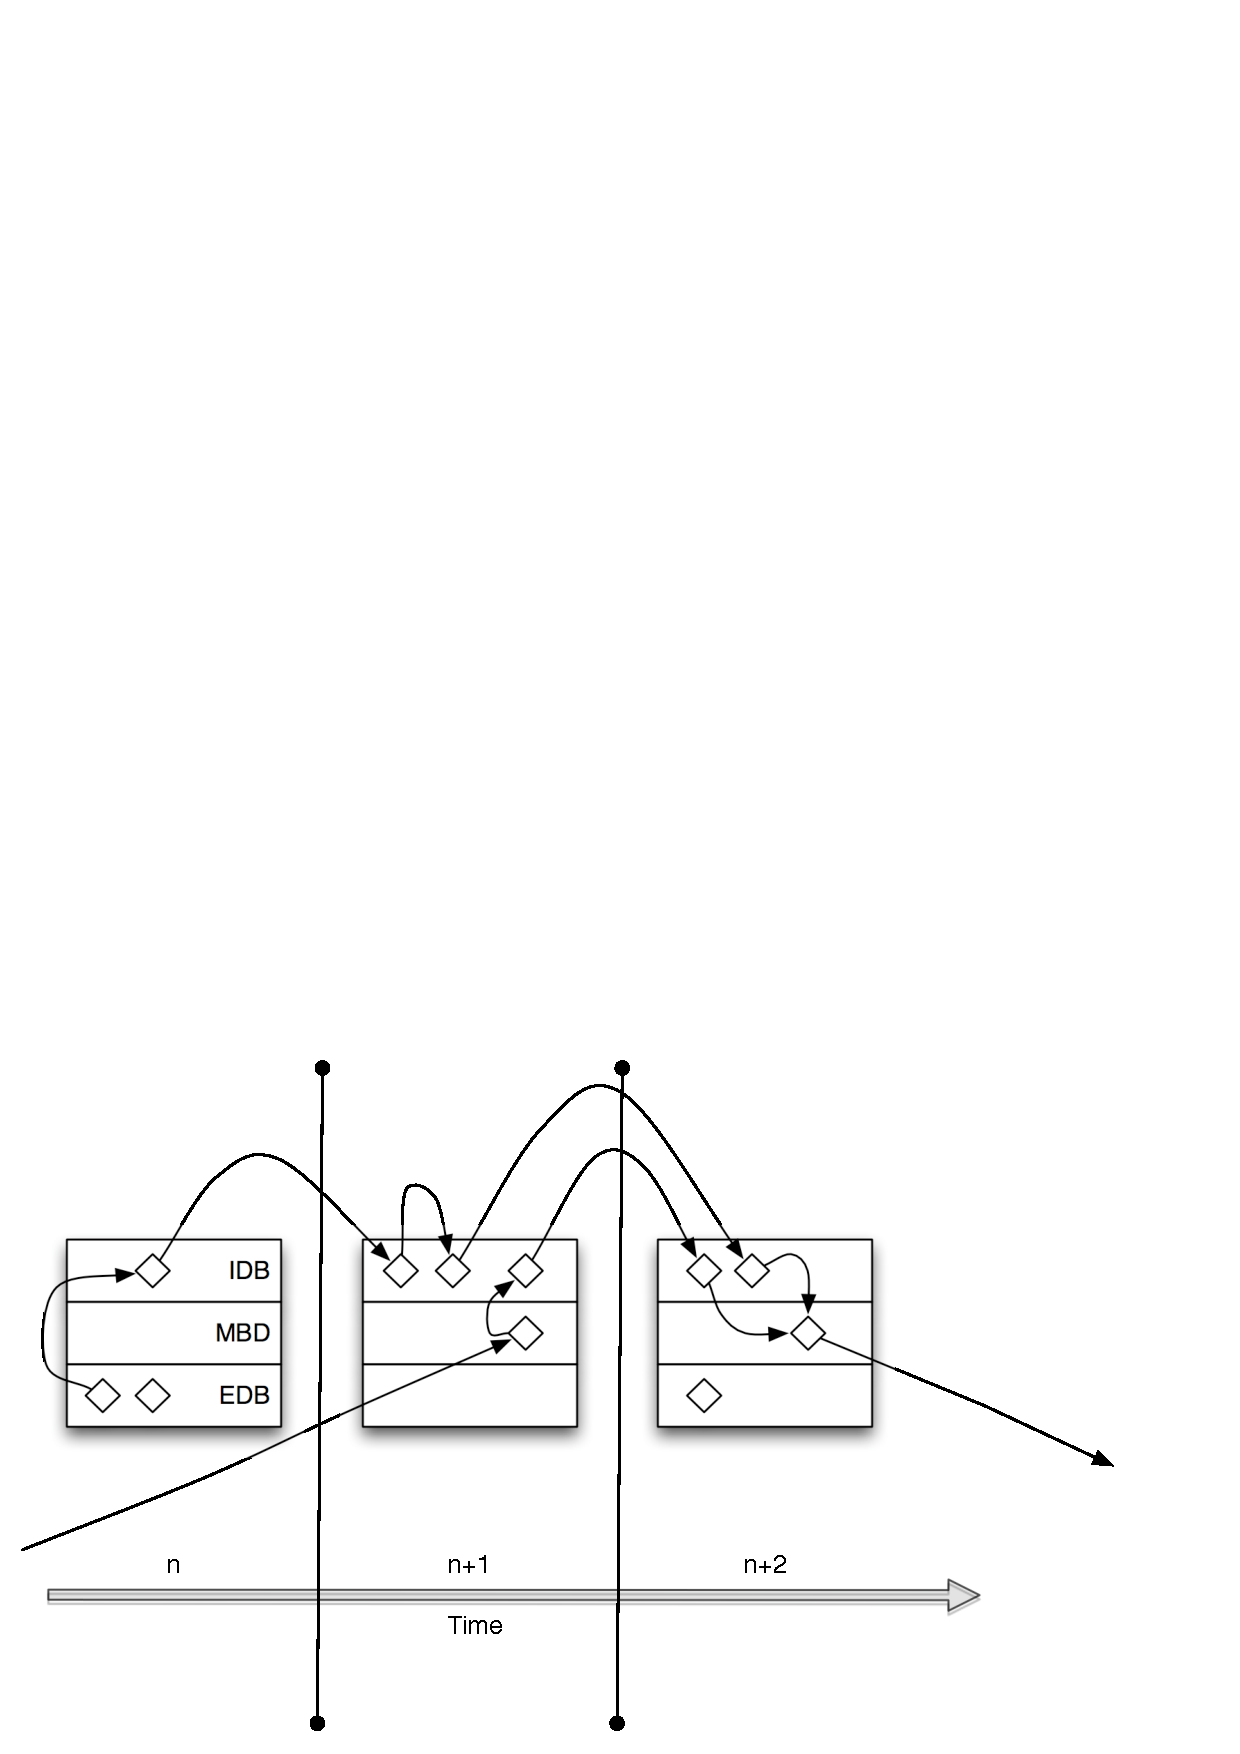
\includegraphics[width=1\linewidth]{figures/edbidbmdb.pdf}
  \label{fig:edbidbmdb}
  \caption{Derivations across time in IDB and MDB relations.}
\vspace{-8pt}
\end{figure}

\paa{this section (its placement \emph{and} content) is somewhat problematic given the current structure
of the draft.  We've established the notion of finite preambles of a (possibly infinite) EDB.  A trace is basically just
an interpretation (a set of ground atoms) -- by calling it a ``trace" we're connoting a post-hoc \wrm{warning: post hoc is undefined} interpretation.
A trace that is just EDB is sufficient, given a program, to augment the trace with IDB and MDB atoms such that
the resulting trace is a model (by simply running a fixpoint computation).  For a program with no async rules, the EDB of input is sufficient to recreate the
program execution exactly -- that is to say, to reproduce the single minimal model of the program given the EDB.
It is \emph{not} sufficient to recreate the execution of a program with async rules: intuitively, we'd need to include in 
the trace the complete MDB, for every entry in it potentially corresponds to one of many possible minimal models.
perhaps we just want to show that there is a method (drop the async rules and run a fixpoint computation to generate
the IDB from MDB and EDB) to regenerate a "complete trace" (ie minimal model) from EDB $\cup$ MDB}

%Consider a non-empty EDB $E$, an empty MBD $M$ and IDB $I$ and a program $P$.  Evaluating $P$ against $E$ may derive facts in $M$ and $I$.

\begin{definition}
A \emph{trace} is any set of facts from the EDB, NDB or IDB of a \lang program evaluation.
\end{definition}

Any trace for a \lang instance $(P,E)$ is an interpretation of $(P,E)$.
%\wrm{lol, why do we need the notion of an incomplete trace?}

\begin{definition}
%
A \emph{complete trace} of an evaluation of a \lang instance is the union of
the given EDB with the derived IDB and MDB.
%
\end{definition}

\begin{lemma}
%
A complete trace of a \lang instance $(P,E)$ is its unique minimal model.
%
\end{lemma}

%\begin{lemma}
%%
%For any bound on $successor$, a complete trace of a \lang  instance $(P,E)$ has a unique minimal model.
%%
%\end{lemma}

If we evaluate E given P, and P is stratifiable, the resulting set of ground atoms is a minimal model.
In our case, however, successor causes our EDB to be infinite, so the minimal model of any \lang program 
with temporal rules is potentially infinite.  \paa{but we'd like to show that a weaker property holds: that for any value $N$
in the \emph{successor} relation, the resulting program has a minimal model.}
\wrm{we either already showed this, or our theorems above are wrong.}


\begin{definition}
A \emph{minimal trace} is a subset of a complete trace that excludes any IDB ground atoms derived through an inductive
rule.
\end{definition}

A minimal trace of a \lang program $P$ is equivalent to the complete trace of which is is a subset -- the latter may be derived from the former by repeated
applications of inductive rules.  However, a given a \lang instance $(P, E)$ and a minimal trace T (where $E \subset T$), a fixpoint
computation will most likely \emph{not} yield a minimal model, because new tuples may be added to the MDB that represent a component 
of a different minimal model, and because these may affect the IDB.  The set of ground atoms $EDB \cup MDB_{old} \cup IDB_{new}$
\emph{may} may be a minimal model, iff $IDB_{new} = IDB_{old}$.  \paa{actually I am not sure if that is true}.  
$(EDB \cup MDB_{old} \cup IDB_{new} \cup IDB_{old})$ is certain to be a model, but is only minimal if $IDB_{new} \subset IDB_{old}$.

A minimal trace records the nondeterminism caused by the delay or reordering of async rules, and
is equivalent to the original program execution.  

\begin{definition}
A \emph{reduced trace} is a minimal trace with normalized time suffixes starting with 0 and increasing by 1 at each step.
\end{definition}

show a (trivial) procedure for reduction and make some claims about equivalences without entanglement.

\begin{definition}
A \emph{event trace} is a \lang EDB.
\end{definition}

An event trace and program P may be used to generate a new IDB and MDB.  The MDB is virtually certain to differ from that of another
execution, while the IDB may differ, depending on its dependency on the MDB.  The union of these three databases is of course a
minimal model, but probably not the same minimal model from another execution.  \paa{but can we say that it will often be true that if we project 
out the time attribute from every predicate, the minimal models will be the same? it won't always be true...}



\subsection{EDB Preambles}

\rcs{I've never seen someone use ``preamble'' to refer to this concept.  Why not call it a prefix?}

A \slang instance's EDB may be arbitrarily large.  In this section we introduce
the notion of a {\em preamble} -- a truncation of the EDB, and prove an
equivalence between full evaluation of a preamble and incremental evaluation
based on evaluation of an earlier preamble.
%A \slang instance may receive arbitrarily many external input tuples over the
%course of its execution, but should not wait arbitrarily long before
%performing deductions.  In this section we introduce the notion of EDB
%preambles, and prove an equivalence between two types of evaluation.

%In general, the EDB of a \slang instance may be infinite, and may lead to unsafe evaluations even when \emph{successor} is derived from it
%as in a post-hoc evaluation.

\begin{definition}
A \emph{preamble} $\alpha_{n}$ of an EDB $\Gamma$ is the set of facts in $\Gamma$ whose timestamp is less than or equal to $n$.
\end{definition}

If the EDB is finite, then it has a maximum timestamp $\top$, \rcs{is successor now part of the EDB? Otherwise, there is no max timestamp} and
$\alpha_{\top}$ = $\Gamma$.  \wrm{I don't think we use $\top$ anywhere else}
Because each preamble is a superset of all preambles with lower indices, we
have the monotonicity property:

$\forall \alpha_{i}, \alpha_{j} \in \Gamma : (i < j) \to (\alpha_{i} \subseteq \alpha_{j})$

%\paa{to your point, bill, I switched the lemma and proof below to one of IDB equivalence in the posthoc vs. continual interpretation
%rather than an inductive proof that every model in the series is minimal.  there is probably a very similar proof of the latter
%that we could include in the next section after introducing minimal models, stratification etc}

\wrm{todo: disuss replacing FP with some derivation tree thing}
\begin{definition}
%
Let $F$ be the set of all finite subsets of possible atoms.  Let $P$ be the set
of all finite subsets of possible rules.  Let $FP : P \times F \mapsto F$ be
the function representing the \emph{fixpoint} computation carried out by a
datalog interpreter.  That is, $FP_p$ takes an EDB to its corresponding IDB.
%
\end{definition}


\begin{lemma}
\label{lem:costmodel}
%
Let $i \in \mathbb{Z}$.  Then, $FP_p(\alpha_{i+1} \cup FP_p(\alpha_i)) =
FP_p(\alpha_{i+1})$.
%
\end{lemma}

%%this could (with some work) lead to an inductive proof
%%that an infinite model is minimal.  we could prove the (weaker?) property that
%%the infinite series of models of increasing finite preambles of an EDB are all 
%%minimal if one of them is.

\begin{proof}

%%Inductive step:

%%if we assume that some program P and finite preamble $\alpha_n$ of a trace $\Gamma$ produce a minimal model, 
%%then it follows that a preamble $\alpha_{n+1}$ and the IDB produced by the previous model produce a minimal model.

by contradiction. Assume $\exists i \in \mathbb{Z}$ such that:
$FP_p(\alpha_{i+1} \cup FP_p(\alpha_i)) \neq FP_p(\alpha_{i+1})$

{\bf Case 1:} $\exists A \in FP_p(\alpha_{i+1} \cup FP_p(\alpha_i)) : A \not\in FP_p(\alpha_{i+1}).$

This implies that $A$ is transitively dependent on atoms in $\alpha_{i+1} \cup
FP_p(\alpha_i)$.  However, if $A$ is transitively dependent only on atoms in
$\alpha_{i+1}$, then $A$ would be in $FP_p(\alpha_{i+1})$.  Thus, $A$ must be
transitively dependent on some atoms in $FP_p(\alpha_{i})$.  But $\alpha_{i}
\subset \alpha_{i+1}$, so this implies that $A$ is transitively dependent on
some atom in $\alpha_{i+1}$, which means $A \in FP_p(\alpha_{i+1})$.  This
contradicts our assumption, thus no such $A$ may exist.

{\bf Case 2:} $\exists A \in FP_p(\alpha_{i+1}) : A \not\in FP_p(\alpha_{i+1} \cup FP_p(\alpha_i)).$

This implies that $A$ is transitively dependent on $\alpha_{i+1}$.  In order
for $A \not\in FP_p(\alpha_{i+1} \cup FP_p(\alpha_i))$, we need $A$ to depend
negatively on an atom $B \in FP_p(\alpha_i)$.  But $B$ transitively depends on
an atom $C \in \alpha_i$.  $C \in \alpha_{i+1}$ by definition (if $B$ is
extensional, then $C=B$), so $B \in FP_p(\alpha_{i+1})$, so $a \not\in
FP_p(\alpha_{i+1})$.  This contradicts our assumption, thus no such $A$ may
exist.
%If $I_2 \neq I_3$, it must be the case that either there exists a ground atom in $I_2$ that is not in $I_3$, or that is in
%$I_3$ and not in $I_2$.  
%Take the former case first.  This means there is an atom $A$ that is entailed by P given $FP(\alpha_{j} \cup FP(\alpha_{i}))$
%but not entailed by P given $\alpha_{j}$, so it must be in $I_1$.   The only circumstances under which an atom in
%$I_1$ would not occur in the IDB $FP(\alpha_{j})$ is if there is a fact $B$ in $\alpha_{j}$ 
%corresponding to a negated subgoal in a rule $r$ in P upon which $A$ depends.  However, for this to occur, because a ground atom 
%in $I_1$ cannot depend upon a ground atom from the ``future", that fact $B$ would need to have occurred at some time less than 
%or equal to the to timestamp of atom $A$.  But this is not possible, because all timestamps in $\alpha_{j}$ that are not in any $\alpha_{k} | k<j$
%are strictly higher than any timestamps in $\alpha_{k}$.  Hence the first case leads to contradiction.
%As for the second case...
\end{proof}

\subsection{Cost Model}
%%\newdef{definition}{Definition}
Lemma~\ref{lem:costmodel} implies that we can trade computation cost for
storage cost in evaluation of a \slang program. 

%In the continuous interpretation of a \slang program, it is in general only
%useful to remember facts at a single timestamp in a predicate.  Two ways to
%approach this issue are to either always persist the ``latest'' version, or
%continuously re-derive the latest version.  These are represented in the naive
%deductive and overwriteable storage implementations below.

%\begin{figure}[t]
%\begin{tabular}{ll} \hline
%%Rule Pattern & Idiom & Prepare & Propose & Election \\ \hline \hline
%$d$ & Cost of a deductive step \\
%$s$ & Cost of storing a tuple \\
%$r$ & Cost of reading a tuple \\ 
%$t$ & Number of tuple derivations from deductive rules \\ 
%\hline
%$S$ & Set of tuples inserted \\
%$U$ & Set of tuples updated \\
%$P$ & Set of stored tuples, with time projected out \\ 
%$T$ & Set of stored tuple timestamps \\ 
%$Q$ & Set of query timestamps \\ \hline 
%\end{tabular}
%\caption{Cost model.}
%\label{fig:breakdown}
%\end{figure}


%\subsubsection{Naive Deductive Implementation}

%To evaluate a trace consisting of $S$ inserts and $U$ updates, a naive
%deductive implementation would:

%\begin{enumerate}
%
%\item
%
%\item
{\bf Naive Deductive Implementation: } We must evaluate every rule at time $1$
through $M$.  This implies persistent storage cost of $|\alpha_M|$, e.g. the
entire preamble up through $M$.
%A bottom-up evaluation of a predicate $P$ consists of evaluating all rules
%that reference $P$ in the head, and may involve polynomially many derivations
%in the size of the EDB up to time $M$.
A naive query plan for execution of a rule $R$ would take the cross product of
all body relations, $CP_R$, select the subset that matches the body conditions,
and project this subset onto the head predicate.  Assume each rule $R$ has an
associated selectivity from the cross product $s_R$, cost per each tuple in the
cross product $d_R$, and cost per each tuple in the subset selected from the
cross product $p_R$.  Each recursion is executed for a certain number of steps
steps.  This step has temporary storage and execution cost of:
%
\[ \sum_{t=0}^M \sum_{R} |CP_{(R,t)}|(p_{(R,t)} \cdot s_{(R,t)} + \cdot
d_{(R,t)}) \]
%
%\end{enumerate}

%In summary, the total execution cost is:

%\[ (S+2U)w + M \cdot \sum_{r : P \in r.head} n_r \cdot s_r \cdot d_r  \]

%Since we only need persist the EDB, the total storage cost is equal to the size
%of the EDB.

%$(|S|+2|U|)s + (|S|+2|U|)r + t + (\displaystyle\sum_{i=0}^{|Q|-1} \displaystyle\sum_{j=0}^{|T|-1} Q_{i} - T_{j})d$

%\subsubsection{Naive Overwriteable Storage Implementation}

%To evaluate a trace consisting of $S$ inserts and $U$ updates, a naive
%deductive implementation would:

%\begin{enumerate}
%
%\item
%Add all $I$ inserts, $D$ deletions, and $U$ updates to a log.  Note that
%an update consists of both an insertion and a deletion.  Assuming that
%inserting a fact into the EDB has some cost $w$ independent of the
%characteristics of the predicate (e.g. all predicates store their facts in hash
%tables), then this step has temporary storage and computation cost $(I+D+2U)w$.

{\bf Naive Overwriteable Storage Implementation: }An overwritable storage
implementation may trade some storage for better execution latency by storing
the most recent version of all predicates.  This implies persistent storage
cost of:
%
\[ |FP(\alpha_{M-1})| + |\alpha_M \cap \alpha_{M-1}| \]

We would need to evaluate every rule $R$ at timestamp $M$.  This entails
temporary storage and execution cost of:
%
\[ \sum_{R} |CP_{(R,M)}|(p_{(R,M)} \cdot s_{(R,M)} + d_{(R,M)}) \]
%This is in contrast to the
%naive deductive model, which would require computation from timestamp 1, but
%would not require persisting the IDB of the most recently computed stratum for
%each predicate.

%In summary, the total execution cost is:

%\[ (S+2U)w + \sum_{r} (M - Q_{r.head}) n_r \cdot s_r \cdot d_r  \]

%The total storage cost is the IDB of each predicate at its most recent
%timestamp.

%%\subsubsection{perhaps we can admit queries over the past that are bounded and pre-stated, and do GC}




\end{document}
